\documentclass{scrartcl}

\usepackage{amsmath}
\usepackage{array}
\usepackage{bytefield}
\usepackage{fontspec}
\usepackage{gitinfo2}
\usepackage{graphicx}
\usepackage{hyperref}
\usepackage{listings}
\usepackage{microtype}
\usepackage{polyglossia}
\usepackage{scrlayer-scrpage}
\usepackage{xcolor}

\linespread{1.3}

\setmainlanguage{lithuanian}

\addtokomafont{disposition}{\rmfamily}

\setmainfont{TeX Gyre Termes}
\setmonofont{TeX Gyre Cursor}

\ohead{Release \gitDescribe\ (\gitCommitterDate)}
\cfoot*{\pagemark}

\newcolumntype{?}{!{\vrule width 1pt}}

\definecolor{lightgray}{gray}{0.8}

\setlength{\headheight}{\baselineskip}
\setlength{\footheight}{\baselineskip}

\lstset{
    basicstyle = \footnotesize\ttfamily,%
    escapeinside = {/*}{*/},%
    firstnumber = 1,%
    numbers = left%
}

\graphicspath{{images/}}

\PolyglossiaSetup{lithuanian}{indentfirst=true}

\begin{document}
    \newcommand{\instr}[3]{\subparagraph{\makebox[6em][l]{\texttt{#1}}} (\texttt{#2})\par#3\par}
    \begin{titlepage}
        \begin{center}
            VILNIAUS UNIVERSITETAS \\
            MATEMATIKOS IR INFORMATIKOS FAKULTETAS \\
            \vspace{4cm}
            \Large\textbf{Multiprograminės operacinės sistemos projektas}
        \end{center}
        \vspace{4cm}
        \begin{flushright}
            \begin{tabular}[t]{l}
                Atliko: 3 kurso studentai \\
                Tautvydas Baliukynas \\
                Edvinas Gervelis \\
                Ernestas Kulik \\
                Justinas Valatkevičius
            \end{tabular}
        \end{flushright}
        \vspace*{\fill}
        \begin{center}
            \large{Vilnius \\ 2018}
        \end{center}
    \end{titlepage}

    \section{Sistemos procesai}
      \subsection{Darbo su procesais primityvai}
      \begin{itemize}
        \item \textbf{KURTIP}
          \par
          Perduodami parametrai:
          \begin{itemize}
            \item Nuoroda į tėvinį procesą
            \item Pradinė proceso būsena (realios mašinos registrų reikšmės ir t.t.)
            \item Perduodamų elementų sąrašas (pvz. operatyvios atminties elementų sąrašas)
            \item Išorinis vardas
          \end{itemize}
          Primityvo veiksmai:
          \begin{itemize}
            \item Sukurtas proceso deskriptorius įtraukiamas į bendrą procesų sąrašą
            \item Deskriptorius įtraukiamas į tėvo sukurtų procesų sąrašą
            \item Priskiriamas vidinis vardas
            \item Sukuriamas naujo proceso vaikinių procesų sąrašas
            \item Sukuriamas naujo procesų sukurtų resursų sąrašas
            \item Procesas įtraukiamas į pasiruošusių procesų sąrašą
          \end{itemize}

        \item \textbf{NAIKINTIP}
          \par
          Perduodami parametrai:
          \begin{itemize}
            \item Proceso išorinis vardas
          \end{itemize}
          Primityvo veiksmai:
          \begin{itemize}
            \item Pašalinti procesą iš visų sąrašų, kuriuose jis yra
            \item Naikinti visus proceso vaikus
            \item Gražinti proceso turėtus pakartotinio panaudojimo resursus
            \item Sunaikinti proceso sukurtus resursus
            \item Naikinti proceso deskriptorių
          \end{itemize}

        \item \textbf{STABDYTIP}
          \par
          Perduodami parametrai:
          \begin{itemize}
            \item Proceso išorinis vardas
          \end{itemize}
          Primityvo veiksmai:
          \begin{itemize}
            \item Proceso būsena pakeičiama į blokuotą sustabdytą arba į pasiruošusią sustabdytą
            \item Jei sustabdytas procesas buvo einamasis, kviečiamas planuotojas
          \end{itemize}

        \item \textbf{AKTYVUOTIP}
          \par
          Perduodami parametrai:
          \begin{itemize}
            \item Proceso išorinis vardas
          \end{itemize}
          Primityvo veiksmai:
          \begin{itemize}
            \item Proceso būsena pakeičiama į pasiruošęs arba blokuotas
            \item Jeigu naujo proceso būsena yra pasiruošęs, kviečiamas planuotojas
          \end{itemize}
      \end{itemize}
      \subsection{Procesų būsenos}
        Procesas visą savo gyvavimo laikotarpį būtinai yra vienoje iš išvardintų būsenų:
          \begin{itemize}
              \item \textbf{Vykdomas} - procesas turi procesorių
              \item \textbf{Blokuotas} - procesas prašo kurio nors resurso, išskyrus procesorių
              \item \textbf{Pasiruošęs} - procesui trūksta vienintelio resurso - procesoriaus
              \item \textbf{Sustabdytas} - procesą sustabdė kažkuris kitas procesas
          \end{itemize}
      \subsubsection{Procesų būsenų kaita}
        \begin{center}
          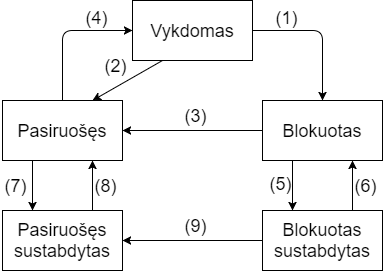
\includegraphics[scale=0.7]{Process_state}
        \end{center}
        \begin{enumerate}
          \item Vykdomas procesas negavo prašomo resurso
          \item Iš vykdomo proceso sistema atima procesorių dėl kokios nors kitos priežasties
          \item Blokuotas procesas gauna reikalingą resursą
          \item Pasiruošęs procesas gauna procesorių
          \item Einamasis procesas sustabdo procesą, kuris buvo užsiblokavęs
          \item Einamasis procesas nuima sustabdymo būsena
          \item Einamasis procesas sustabdo procesą, kuris buvo pasiruošęs
          \item Einamasis procesas nuima sustabdymo būseną
          \item Užsiblokavęs sustabdytas procesas gauna reikalingą resursą
        \end{enumerate}
      \subsection{Procesų kūrimas}
      Procesai yra skirstomi į sisteminius ir vartotojo. Sisteminiai procesai yra sukuriami sistemos darbo pradžioje. Juos sukuria procesas \textbf{StartStop}. Vartotojo procesai yra sukuriami sisteminių procesų. Bendra procesų kūrimo schema:
      \begin{center}
        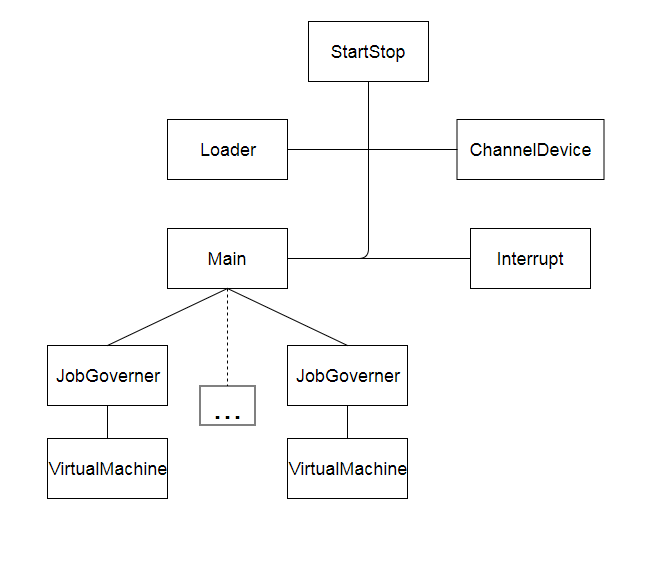
\includegraphics[scale=0.5]{Process_creation}
      \end{center}
       \subsection{Vartotojo programos patekimas į sistemą}
        Kol vartotojo programa iš baitų išorinėje atmintyje tampa procesu operacinėje sistemoje, jai tenka pereiti kelis etapus. Visų pirma yra kviečiamas procesas Loader, kuris iš išorinės atminties perskaito užduoties programą, kurią konvertuoja į procesoriui suprantamą formatą ir siunčia pranešimą procesui Main, kuris sukuria po naują JobGovernor procesą kiekvienai vartojo užduočiai. Galiausiai JobGovernor sukuria VirtualMachine procesą, kuris jau gali vykdyti vartojo programą.
        \begin{center}
          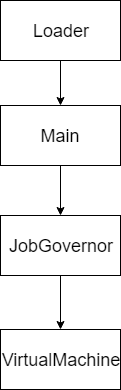
\includegraphics[scale=0.5]{Program_load}
        \end{center}

      \subsection{Procesų veikimas}
        \subsubsection{StartStop}
          StartStop yra pirmas procesas, kuris atsiranda sistemoje, vos tik ją paleidus. Jo paskirtis yra sukurti visus kitus sisteminius procesus bei resursus kurie leistų vykdyti operacinės sistemos darbą. Atlikęs savo užduotį StartStop procesas užsiblokuoja laukdamas "OS pabaiga" resurso, kuris bus atlaisvintas tik tada, kai operacinė sistema norės pabaigti savo darbą, taigi, beveik visą OS veikimo trukmę, procesas StartStop bus užsiblokavęs. Kai galiausiai jis atsiblokuos sulaukęs "OS pabaiga" resurso, jis sunaikins savo sukurtus sisteminius procesus bei resursus ir operacinės sistemos darbas bus baigtas.
          \begin{center}
            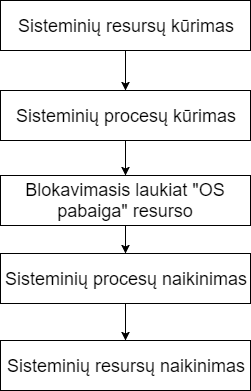
\includegraphics[scale=0.5]{StartStop}
          \end{center}

      \subsubsection{Loader}
        Procesas Loader yra svarbiausias procesas vartojo užduoties patekimo į operacinę sistemą schemoje. Jis pradeda savo darbą laukdamas "Iš vartotojo sąsajos" resurso, kuris bus atlaisvintas tuomet, kai operacinės sistemos vartotojas nurodys, kurią programą jis nori įvykdyti. Tuomet bus atlaisvintas Loader procesui reikalingas resursas ir vartotojo programa bus nuskaityta iš išorinės atminties. Analizuodamas nuskaitytus duomenis, procesas Loader priima sprendimą, kiek vartotojo atminties resursų reikės ir blokuojasi laukdamas, kol resursai bus gauti. Gavęs vartotojo atminties resursą, Loader perkels vartotojo programą į nurodytą atminties vietą ir pasiųs pranešimą procesui Main.
        \begin{center}
          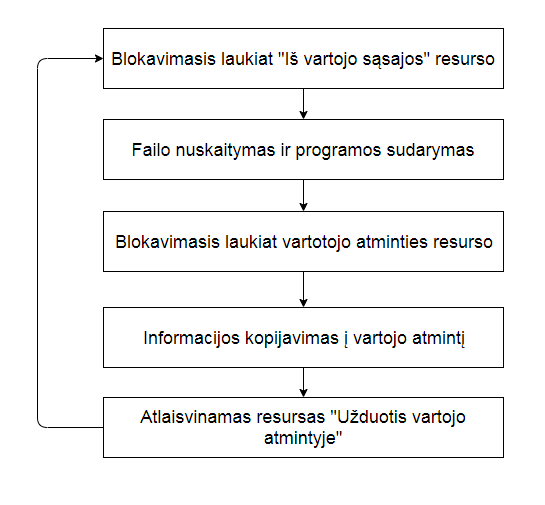
\includegraphics[scale=0.5]{Loader}
        \end{center}
      \subsubsection{Main}
        Procesas Main darbą pradeda užsiblokavęs ir laukdamas, kol gaus pranešimą iš "Užduotis vartotojo atmintyje". Šį pranešimą procesas Main gali gauti dviem atvejais:
        \begin{enumerate}
          \item Iš proceso loader. Tai reiškia, kad sistemai buvo užduota įvykdyti naują vartotojo programą. Šiuo atveju reikia sukurti naują JobGovernor procesą ir blokuotis laukiant kito "Užduotis vartotojo atmintyje" pranešimo.
          \item Iš proceso JobGovernor. Šis pranešimas turėtų būti fiktyvus ir reikšti, kad VirtualMachine procesas, už kurį buvo atsakingas resursą atlaisvinęs JobGovernor procesas, baigė savo darbą ir JobGovernor turi būti sunaikintas.
        \end{enumerate}
        \begin{center}
          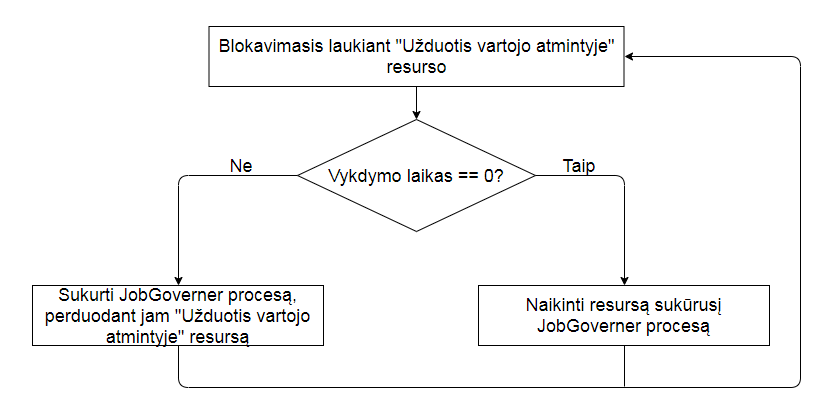
\includegraphics[scale=0.5]{Main}
        \end{center}
      \subsubsection{Interrupt}
        Procesas Interrupt pradeda darbą laukdamas "Pertraukimas" resurso. Šis resursas atlaisvinamas kai VirtualMachine, vykdydamas vartojo programa susiduria su situacija, kurios pats negali apdoroti. Tuomet Interrupt procesas nustato, kokia situacija kilo vykstant VirtualMachine procesui, suranda kuris JobGovernor procesas yra atsakingas už VirtualMachine, kuriame kilo pertraukimas ir būtent tam JobGovernor procesui perduoda "Iš pertraukimo" pranešimą. Taigi, šio proceso paskirtis, leisti VirtualMachine procesui bendrauti su JobGovernor procesu.
        \begin{center}
          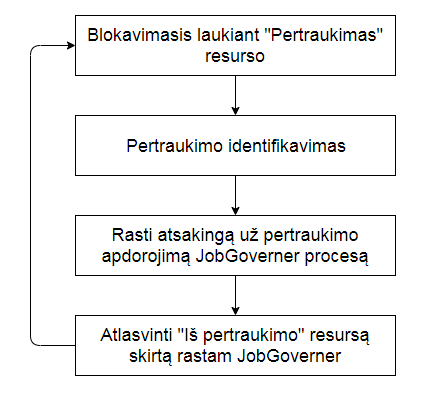
\includegraphics[scale=0.5]{Interrupt}
        \end{center}
      \subsubsection{ChannelDevice}
        ChannelDevice procesas leidžia kitiems procesams apsikeisti duomenimis tarp įrenginių ir realios mašinos atminties. Kadangi realios mašinos kanalų įrenginys vienu metu gali atlikti vieną duomenų perdavimą, mes turime užtikrinti, kad proceso ChannelDevice vienu metu nenaudos keli procesai. Todėl ChannelDevice pradeda darbą atlaisvindamas "Channel Device" resursą ir laukdamas, kol gaus "Data Transfer" pranešimą. Šį pranešimą kanalų įrenginiui turėtų atsiųsti procesas, kuris prieš tai blokavosi laukdamas "Channel Device" resurso ir jį gavęs pasiuntė "Data Transfer" pranešimą. Su "Data Transfer" pranešimu ChannelDevice procesas gauna visą reikalingą informaciją, kad galėtų atlikti duomenų persiuntimą per kanalų įrenginį. Tada nurodo kanalų įrenginiui ką daryti ir pabaigęs savo darbą atlaisviną "From Channel Device" pranešimą, kurio turėtų laukti duomenų perdavimą iniciavęs procesas.
        \begin{center}
          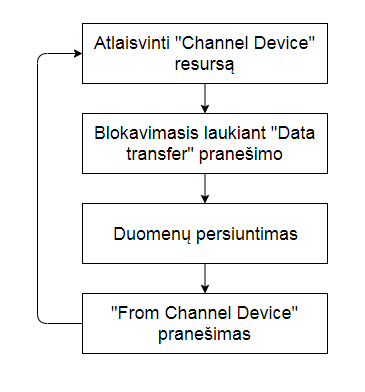
\includegraphics[scale=0.5]{ChannelDevice}
        \end{center}

      \subsubsection{JobGovernor}
        JobGovernor procesas yra atsakingas už VirtualMachine proceso sukūrimą ir aptarnavimą. Sukūręs VirtualMachine procesą, JobGovernor užsiblokuoja ir laukia, kol sukurtajame VirtualMachine procese kils pertraukimas ir bus atlaisvintas "Iš pertraukimo" resursas (jį atlaisvina procesas Interrupt). Gavęs šį resursą JobGovernor sustabdo VirtualMachine proceso veikimą ir pradeda pertraukimo analizę. Visų pirma yra patikrinama, ar pertraukimas buvo įvedimo/išvedimo, jeigu taip, tai nustatoma, kokia konkrečiai įvedimo/išvedimo operacija buvo vykdoma ir per kanalų įrenginį atliekamas duomenų perdavimas. Jeigu vis dėlto pertraukimas nebuvo įvedimo/išvedimo, tuomet gali būti, kad virtualioje mašinoje TI registras pasiekė nulinę reikšmę. Tokiu atveju TI registras atnaujinamas ir VirtualMachine procesas vėl iš naujo konkuruoja su kitais procesais dėl procesoriaus. Tačiau, jeigu tai nebuvo nei įvedimo/išvedimo nei timeout pertraukimas, reiškia, kad virtualioje mašinoje įvyko kažkokia klaida ir jos darbas turi būti baigtas. O kadangi JobGovernor yra atsakingas už mašinos prižiūrėjimą, tai šis procesas daugiau nebeturi prasmės egzistuoti, todėl siunčia fiktyvų pranešimą procesui Main, kuris gali sunaikinti JobGovernor.
        \begin{center}
          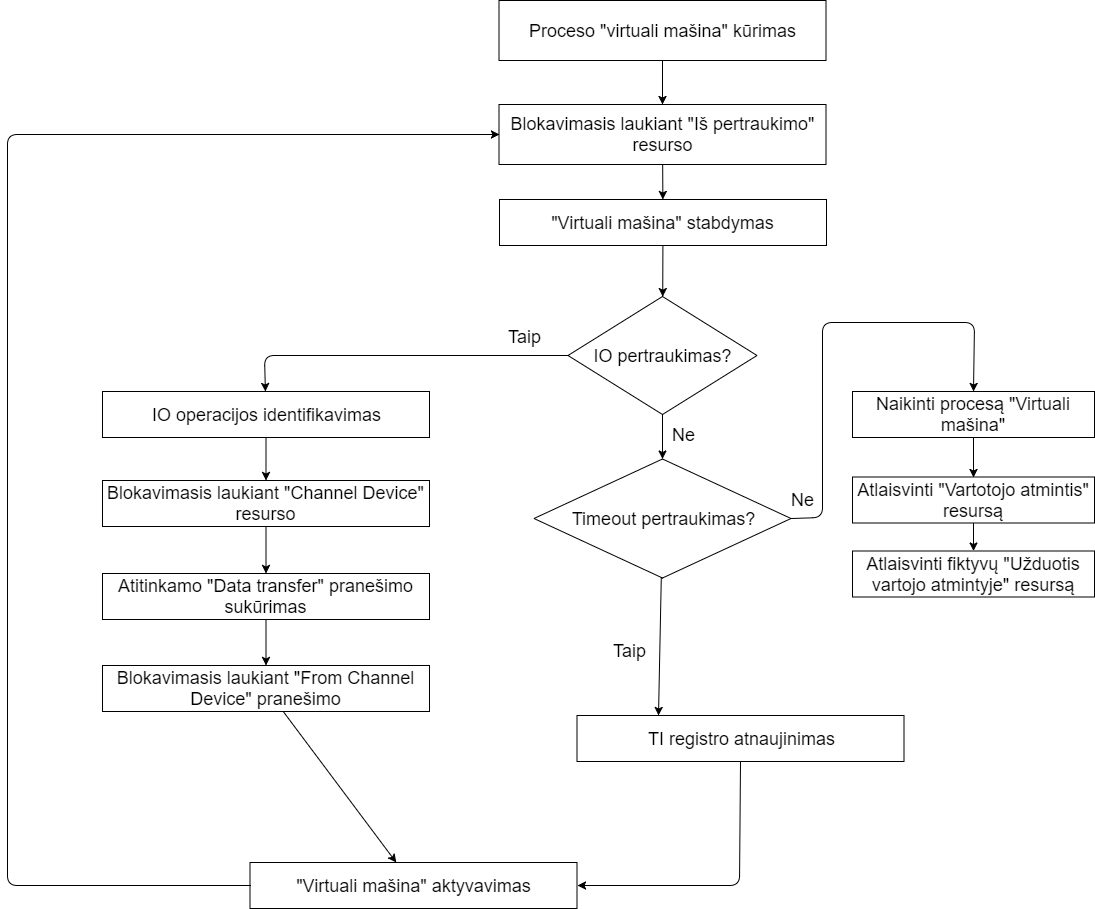
\includegraphics[width=\textwidth]{JobGovernor}
        \end{center}

      \subsubsection{VirtualMachine}
        Šis procesas yra skirtas vartotojo programos vykdymui.
        \begin{center}
          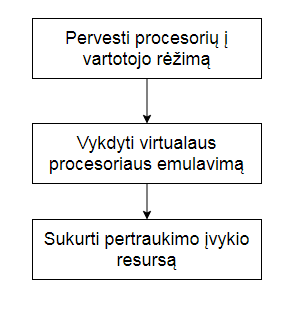
\includegraphics[scale=0.5]{VirtualMachine}
        \end{center}

    \section{Resursai}
      Sistemoje turime dviejų tipų resursus:
      \begin{enumerate}
        \item Statiniai - atmintis, procesorius bei kiti, kurie gyvuoja visą sistemos darbo laiką
        \item Dinaminiai - resursai, kuriuos kuria procesai savo darbo eigoje. Tokie resursai gali būti naudojami kaip pranešimai apie kažkokius sistemoje vykstančius įvykius.
      \end{enumerate}
      Darbui su resursais sistemoje yra naudojami tokie primityvai:
      \begin{itemize}
        \item \textbf{KURTIR}
          \par
          Perduodami parametrai:
          \begin{itemize}
            \item Nuoroda į resursą sukūrusį procesą
            \item Resurso išorinis vardas
          \end{itemize}
          Primityvo veiksmai:
          \begin{itemize}
            \item Pridedamas prie bendro resursų sąrašo
            \item Pridedamas prie tėvo sukurtų resursų sąrašo
            \item Prisikiriamas unikalus vidinis vardas
            \item Sukuriamas resurso elementų sąrašas
            \item Sukuriamas laukiančių procesų sąrašas
          \end{itemize}

        \item \textbf{NAIKINTIR}
          \par
          Perduodami parametrai:
          \begin{itemize}
            \item Resurso išorinis vardas
          \end{itemize}
          Primityvo veiksmai:
          \begin{itemize}
            \item Resurso deskriptorius išmetamas iš tėvo sukurtų resursų sąrašo
            \item Naikinamas resurso elementų sąrašas
            \item Atblokuojami visi resurso laukiantys procesai
            \item Resursas išmetamas iš bendro resursų sąrašo
            \item Naikinamas resurso deskriptorius
          \end{itemize}

        \item \textbf{PRAŠYTIR}
          \par
          Perduodami parametrai:
          \begin{itemize}
            \item Resurso išorinis vardas
            \item Kokios resurso dalies prašoma
          \end{itemize}
          Primityvo veiksmai:
          \begin{itemize}
            \item Iškvietęs procesas užblokuojamas ir įtraukiamas į resurso laukiančių procesų sąrašą
            \item Kviečiamas resursų paskirstytojas
          \end{itemize}

        \item \textbf{ATLAISVINTIR}
          \par
          Perduodami parametrai:
          \begin{itemize}
            \item Resurso išorinis vardas
            \item Atlaisvinamas resurso elementas
          \end{itemize}
          Primityvo veiksmai:
          \begin{itemize}
            \item Resurso elementas pridedamas prie resurso elementų sąrašo
            \item Kviečiamas resursų paskirstytoja
          \end{itemize}
      \end{itemize}
      \subsection{Resursų lentelė}
      \begin{center}
        \begin{tabular}{ | l | l | l | l |}
          \hline
            Resurso pavadinimas & Sukuria & Laukia & Atlaisvina\\
            \hline
            OS pabaiga          & Sistemine Komanda shutdown & StartStop &-\\
            IsVartotojoSasajos  & Sistemine Komanda load  & Loader &-\\
            VartojoAtmintis     & StartStop     & Loader & JobGovernor\\
            UzduotisVartotojoAtmintyje & Loader & Main &-\\
            Pertraukimas        & VirtualMachine& Interrupt &-\\
            IsPertraukimo       & Interrupt     & JobGovernor&-\\
            ChannelDevice       & StartStop & JobGovernor & ChannelDevice \\
            DataTransfer        & JobGovernor   & ChannelDevice &-\\
            FromChannelDevice   & ChannelDevice & JobGovernor&-\\

          \hline
        \end{tabular}
        \end{center}
      \subsection{Resursų paskirstytojas}
        Resursų paskirstytojo užduotis - tikrinti konkretaus resurso laukiančių procesų sąrašą ir esant galimybei perduoti resursą laukiančiam procesui ir pažymėti jį kaip pasiruošusį (arba pasiruošusį sustabdytą, jeigu pereinama iš būsenos blokuotas sustabdytas).
        \subsubsection{Planuotojas}
        Procesorius iš esmės yra vienas iš sistemos resursų, tačiau, šio resurso svarba sistemoje yra milžiniška, todėl procesorius turi savo atskirą resursų paskirstytoją - planuotoją.
        \par
        Planuotojo pagrindinė užduotis yra skirstyti procesorių sisteminiams ir vartotojo procesams. Skirstymas remiasi procesų prioritetais - planuotojas stengiasi procesorių atiduoti procesui, kurio prioritetas yra aukščiausias.
        \par
        Plantuojo veikimas pagrįstas šia schema:
        \begin{center}
          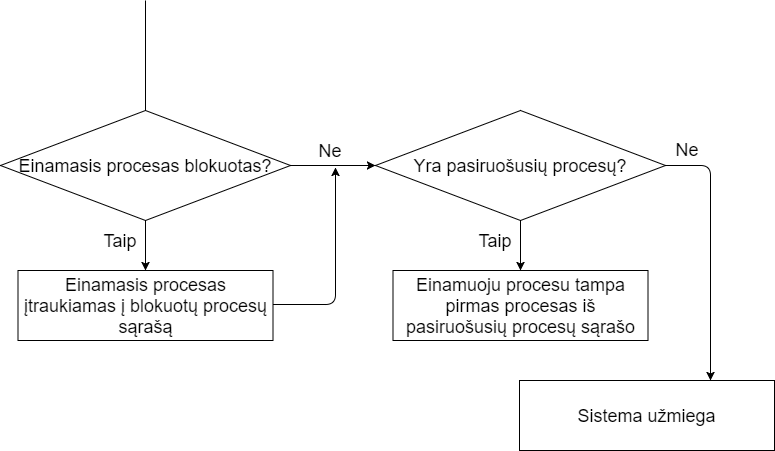
\includegraphics[width=\textwidth]{Planner}
        \end{center}
        Žingsnis, kurio metu procesas iš pasiruošusių procesų sąrašo tampa einamuoju procesu susideda iš tokių veiksmų:
        \begin{enumerate}
          \item Išsaugoma einamojo proceso aplinka, kad ateityje būtų įmanoma pratęsti vykdytą procesą
          \item Užkraunama naujo einamojo proceso aplinka
          \item Naujas einamasis procesas pažymimas kaip einamasis
        \end{enumerate}
        \begin{thebibliography}{999}
            \bibitem{}
                Giedrius Šiaulys,
                Magistro darbas. Mokomoji operacinė sistema,
                2003.
        \end{thebibliography}
    \end{document}
